\documentclass{sciposter}
\usepackage{lipsum}
\usepackage{epsfig}
\usepackage{amsmath}
\usepackage{amssymb}
\usepackage{multicol}
\usepackage{graphicx,url}
\usepackage[portuges, brazil]{babel}  
\usepackage[utf8]{inputenc}
\usepackage{listings}
\usepackage{color}
\usepackage{indentfirst}

\lstset{language=C++,
                basicstyle=\ttfamily,
                keywordstyle=\color{blue}\ttfamily,
                stringstyle=\color{red}\ttfamily,
                commentstyle=\color{green}\ttfamily,
                morecomment=[l][\color{magenta}]{\#}
}
%\usepackage{fancybullets}
\newtheorem{Def}{Definition}


\title{Uma implementação do jogo Pedra, Papel e Tesoura utilizando Visão Computacional}
%Título do projeto

\author{Ezequiel França dos Santos, Gabriel Fontenelle Senno Silva}

\institute
{Bacharelado em Ciência da Computação\\
Centro Universitário SENAC - Campus Santo Amaro
  (SENAC-SP)\\
  Av. Engenheiro Eusébio Stevaux, 823 -- Santo Amaro, São Paulo -- CEP 04696-000 -- SP -- Brasil}
%Nome e endereço da Instituição

\email{{ezefranca.br,colecionador.gabriel},{(@gmail.com})}
% Onde você coloca os emails dos integrantes


%\date is unused by the current \maketitle

\rightlogo[1]{Ecomp-logo}
\leftlogo[1]{Senac-logo}
% Exibe os logos (direita e esquerda)
% Procure usar arquivos png ou jpg, e de preferencia mantenha na mesma pasta do .tex
%%%%%%%%%%%%%%%%%%%%%%%%%%%%%%%%%%%%%%%%%%%%%%%%%%%%%%%%%%%%%%%%%%%%%%%%%%%%%%%%
%%% Begin of Document



\begin{document}
%define conference poster is presented at (appears as footer)

\conference{{\bf BCC 15 anos}, 5º Projeto Integrador III - 15 anos do Bacharelado em Ciência da Computação, Senac, 27 de Novembro de 2013, São Paulo, Brasil}

%\LEFTSIDEfootlogo 
% Uncomment to put footer logo on left side, and
% conference name on right side of footer

% Some examples of caption control (remove % to check result)

%\renewcommand{\algorithmname}{Algoritme} % for Dutch

%\renewcommand{\mastercapstartstyle}[1]{\textit{\textbf{#1}}}
%\renewcommand{\algcapstartstyle}[1]{\textsc{\textbf{#1}}}
%\renewcommand{\algcapbodystyle}{\bfseries}
%\renewcommand{\thealgorithm}{\Roman{algorithm}}

\maketitle

%%% Begin of Multicols-Enviroment
\begin{multicols}{3}

%%% Abstract
\begin{abstract}
Este projeto consiste em 2 jogos controlados por aglortimos de Visão Computacial  Diferetnes. Um dos jogos tem como base a identificação das cores primarias e o outro em uma rustica detecção de face atraves de uma detecção de bordas sobre a imagem.

\end{abstract}

%%% Introduction
\section{Introducão}
Jogos interativos tem sido uma grande area a ser explorada a medida que a tecnologia e as formas de fazer jogos avançam. A partir disso e buscando uma interação com a camera , chegamos ao nosso 
trabalho ,  que tem como foco criar jogos que posibilitem uma interação agradavel com a camera , sendo ela um dispositivo essecial para a jogabilidade e a ate para a diversao do ususario , de forma que ela nao atrapalhe ou se torne algo discartavel para o jogador.

\newcommand{\imsize}{0.45\columnwidth}




\section{Objetivos}
Nesse projeto tivemos 2 objetivos diferentes a serem alcançados nos 2 jogos que criamos. 

Para o primeiro jogo , o principal objetivo era reconhecer com precisão 4 cores , verde , amarelo , vermelho e azul , assim conseguimos estruturar o classico jogo genius baseado nas imagens reconhecidas pela camera.

O segundo jogo ja foi algo pouco mais complexo pois envolveu mais algoritimos como detecções de borda , e alguns filtros , e tem como objetivo uma rustica detecção de face , baseada nas bordas 
que podem ser reconhecidas na face como boca e os olhos , provendo um reconhecimento eficiente e com alguma precisão.

\section{Metodologia}
Para o inicio do trabalho fomos introduzidos a uma mini biblioteca , baseada em OpemCV que seria a nossa unica ferramenta de acesso a camera e ao tratamento das imagens , sendo ela bem simples
a maior parte do trabalho de tratamento e reconhecimento nas imagens foi feito por nos mesmos. A biblioteca nos disponibilizou basicamente funções de acesso a imagem da camera , sendo a que
principal delas era a que capturava a imagem da camera e a transformava em uma matriz tridimensional onde as colunas x e y representavam cada pixel da imagem e dentro de cada x e y existiam 3 
campos que sao respectivamente os componetes R (vermelho) G (verde) e B(azul) de cada pixel .

\subsubsection*{Jogo Genius}

A Principal ideia do reconhecimento das cores desse jogo foi baseada na basica detecção de vermelho , onde verificamos se o componente R do pixel é maior que a soma dos outros dois G e B.
Esse metodo funciona bem para o vermelho , porem uma variante dele para as outras cores que precisavamos detectar nao funcionou muito bem ,devido a pequenas mudanças de luz  e algumas interferencias , entao tivemos que partir para alguma outra soluçao.
Depois de pesquisar  , concluimos que mudando o espaço de cor R B G para o H S V, onde o H representa a cor em si , o S a saturação dessa cor e o V o brilho , com esse espaço de cor , diferente do RGB , conseguimos definir claramente um range para cada tipo de cor , podendo filtrar com sucesso as cores que nos desejavamos.
\\
\\
O algoritmo usado para a Conversão

\begin{figure}[ht]
\centering
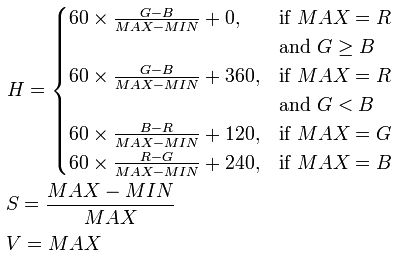
\includegraphics[width=8in]{img4.png}
\end{figure}

\\
\\


Um Exemplo de resultado com Azul

\begin{figure}[ht]
\centering
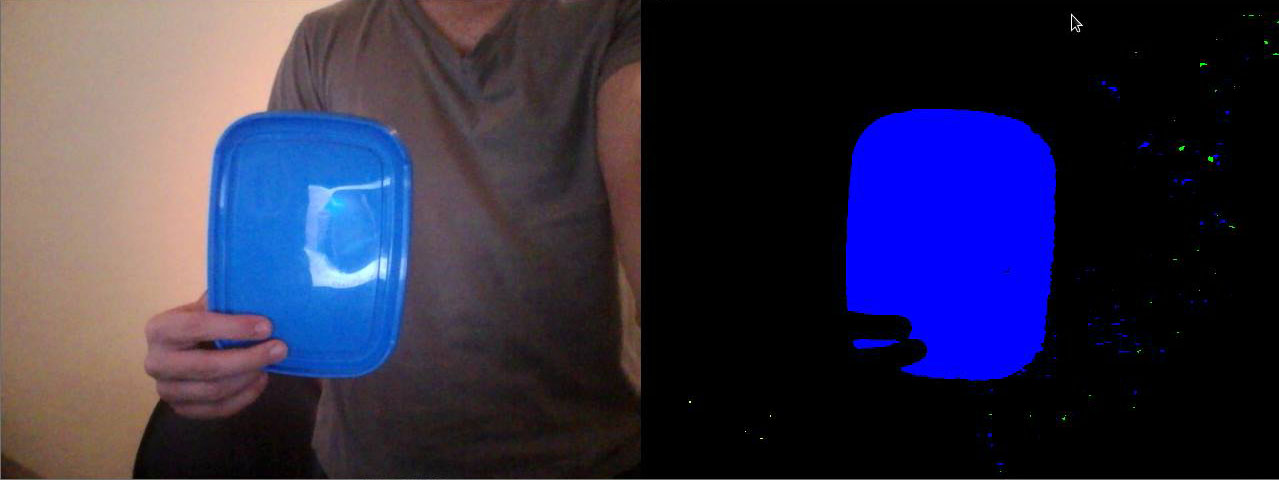
\includegraphics[width=8in]{img2.jpg}
\end{figure}


\subsubsection*{Jogo do Vini}





\subsubsection{Binarização da imagem}

Existem diversos algoritmos para binarização de imagens, dentre a lista de soluções para este  o algoritmo de Otsu, por ser de fácil implementação e apresentar resultados satisfatórios nos experimentos realizados.

O método de Otsu é um método de \textit{thresholding} global, isto é, o valor obtido é
uma constante, para escolha do melhor limiar. A base deste método é sua interpretação
do histograma como como uma função de densidade de probabilidade
discreta \cite{Limiar}, da seguinte maneira:

\begin{equation}\label{eq:histograma_norm}
  p_r(r_q) = \frac{n_q}{n}, q = 0, 1, 2, ..., L-1
\end{equation}

Onde:

\begin{itemize}
  \item $ n $ é o total de \textit{pixels} da imagem;
  \item $ n_q $ é o total de \textit{piixels} que tem intensidade $ r_q $ e
  \item $ L $ é o total de níveis de intensidade na imagem.
\end{itemize}

O resultado da binarização com limiar ajustado segundo o método de Otsu pode
ser observado na Figura \ref{fig:bin_otsu}

\begin{figure}[ht]
\centering
\mbox{\subfigure{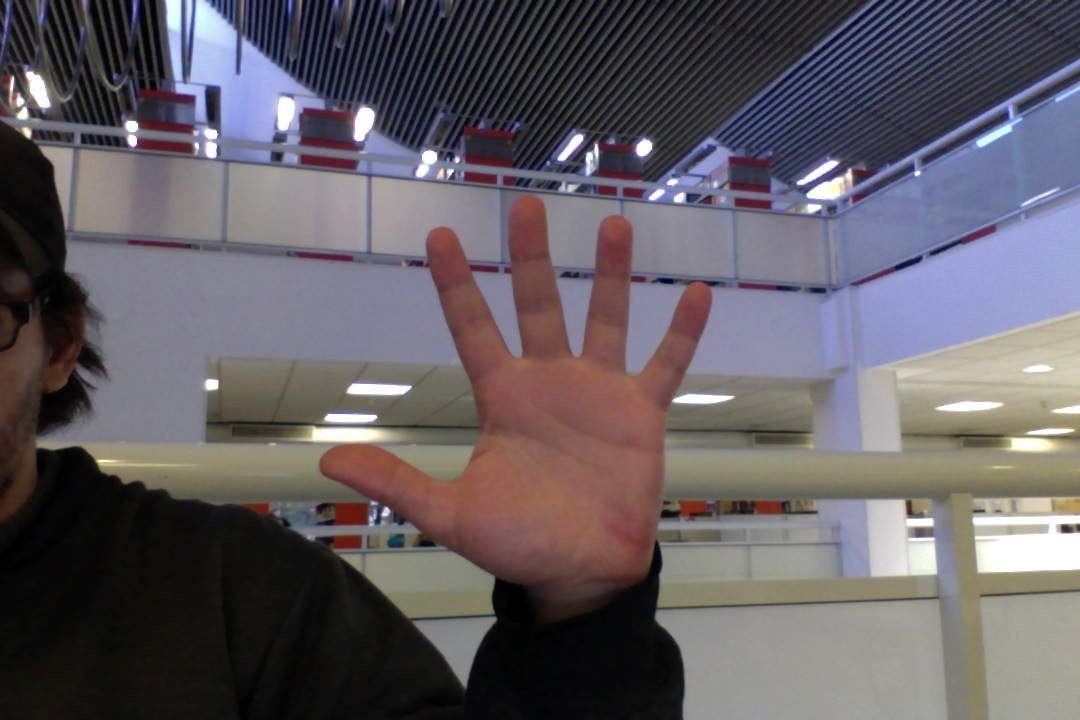
\includegraphics[width=3in]{normal.jpg}}\quad
\subfigure{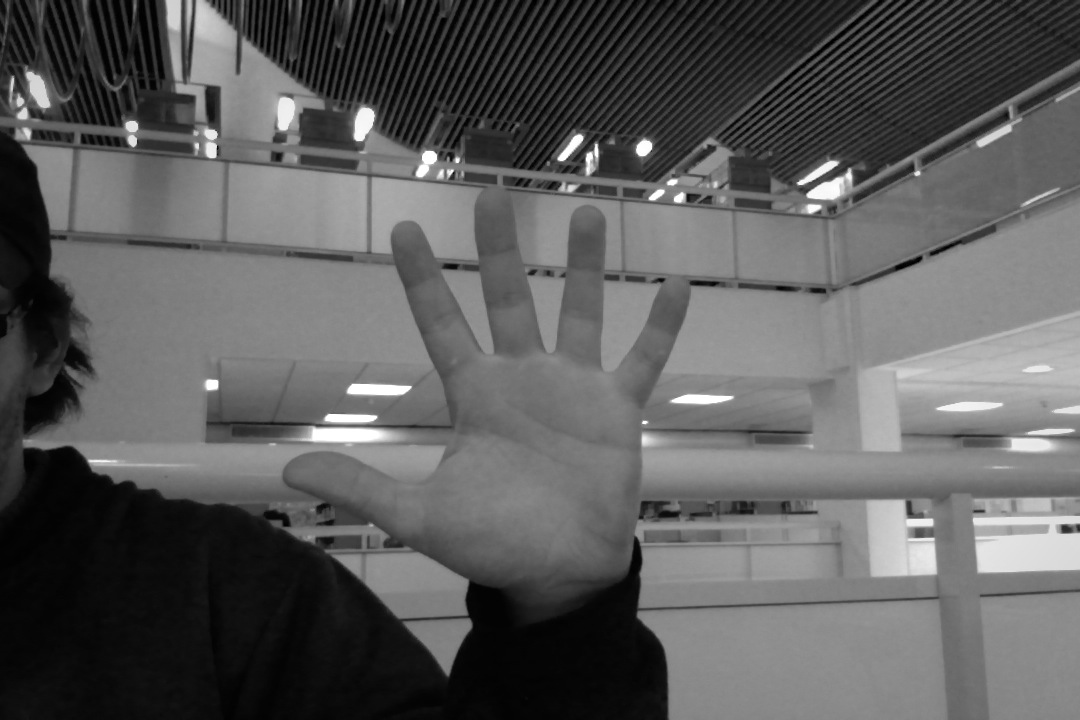
\includegraphics[width=3in]{cinza.jpg} }}
\caption{ Imagem binarizada com limiar definito pelo método de Otsu. }
\label{fig:bin_otsu}
\end{figure}

\subsubsection*{Detecção de bordas com filtro Sobel}

O filtro Sobel calcula o gradiente da intensidade da imagem em cada ponto, dando a direcção da maior variação de claro para escuro e a quantidade de variação nessa direcção, através de duas matrizes 3x3, que são convoluídas com a imagem original para calcular aproximações das derivadas - uma para as variações horizontais $Gx$ e uma para as verticais $Gy$.
\begin{center}{Máscara de Sobel 3x3}
$$
Gx=\left[\begin{array}{rrr}
-1&0&+1\\
-2&0&+2 \\
-1&0&+1
\end{array}\right]\quad
Gy=\left[\begin{array}{ccc}
-1&-2&-1\\
0& 0& 0 \\
+1&+2&+1
\end{array}\right]
$$
\end{center}
A magnitude do gradiente é dado por:

$$
|G|=\sqrt{Gx^2 + Gy^2}
$$	

\subsection*{Reconhecimento dos padrões}
\subsubsection*{Determinação do fecho convexo}


\bigskip
\subsubsection*{Algortimo da embrulho de presente}

\begin{itemize}

\item O {\em algoritmo da marcha de Jarvis}, popularmente conhecido como {\em gift
wrapping algorithm / algoritmo do embrulho de presente} , visita os pontos do fecho convexo de maneira ordenada.

\begin{enumerate}

\item Começamos com qualquer ponto do fecho. O ponto com maior coordenada em x é uma escolha natural. Chamamos esse ponto de $(X_0, Y_0)$.

\item Varremos ("marchamos") através de todos os pontos $(X_i, Y_i)$ e localizamos o ponto tal que o ângulo a partir da coordenada $(1,0)$ para $(X_i - X_0, Y_i - Y_0)$ é minímo.
TEste é o próximo ponto de sentido anti-horário a partir de $(X_0,Y_0)$ no fecho, chamamos-o de $(X_1, Y_1)$.

\item Suponhamos que tenhamos localizado o ponto $(X_i,Y_i)$, $i=1, \ldots, m$ que ocorrem no sentido anti-horário ao fecho onde $m \ge 2$.
Calculamos todos os ângulos entre os vetores $(X_i - X_m, Y_i - Y_m)$ e
$(X_{m-1} - X_m, Y_{m-1} - Y_m)$, e procuramos o ponto $i$ que tenha o menor âgulo positivo.  Adicionamos este ponto ao fecho.

\item Retornarmos a etapa 3 até que $(X_m,Y_m) = (X_0,Y_0)$.

\end{enumerate}

\begin{center}
\scalebox{.7}{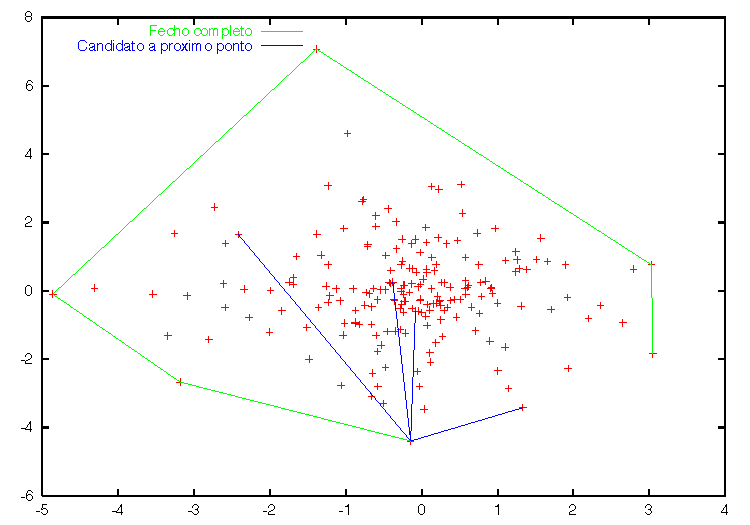
\includegraphics{figura7.pdf}}
\end{center}

\item O algoritmo de marcha Jarvis tem no pior caso complexidade O($n^2$), o que ocorre se todos os pontos estão no fecho. Em geral, se $h$ pontos estã no fecho, a complexidade é O($nh$).


\end{itemize}


\section{Resultados e Discussão}

Verificar os principais resultados obtidos de acordo com os objetivos propostos.\\

Nacken \cite{Nacken:thesis} derived an algorithm for computation
of pattern spectra for granulometries based on openings by discs of increasing
radius for various metrics, using the opening transform. After the
opening transform has been computed, it is straightforward to compute the
pattern spectrum:
\begin{itemize}
\item Set all elements of array {\tt S} to zero
\item For all $x \in X$ increment {\tt S}[$\Omega_X(x)$] by one.
\end{itemize}

To compute the pattern \emph{moment} spectrum, the only thing that needs to be
changed is the way {\tt S}[$\Omega_X(x)$] is incremented. As shown in Algorithm
\ref{alg:spect}.

\begin{algorithm}
\begin{itemize}
\item Set all elements of array {\tt S} to zero
\item For all $(x,y) \in X$ increment {\tt S}[$\Omega_X(x,y)$] by
$x^iy^j$.
\end{itemize}
\caption{ Algorithm for computation of pattern moment
spectrum of order $ij$. \label{alg:spect}}
\end{algorithm}

This algorithm can
readily be adapted to other granulometries, simply by computing the
appropriate opening transform.

\begin{figure}
\begin{center}
\begin{tabular}{c c}

\end{tabular}
\end{center}
\caption{ \label{fig:tauspect}
The opening transform using city-block metric: (a) opening transform of
Fig. 1(c); (b) pattern spectrum; (c) pattern variance-$x$;
(d) variance-$y$ spectra.}
\end{figure}


\renewcommand{\imsize}{0.3\columnwidth}
\begin{figure}
\begin{center}
\end{center}
\caption{ \label{fig:binspect} Pattern mean-$x$ (top) and variance-$x$
(bottom) spectra: the three collumns show spectra for Fig. 1(a), (b) and (c)
from left to right respectively.  Unlike the standard pattern spectra,
these spatial pattern spectra can distinguish the three images.}
\end{figure}

\section{Conclusão}

Sitting on a corner all alone,
staring from the bottom of his soul,
watching the night come in from the window
\\
It'll all collapse tonight, the fullmoon is here again
In sickness and in health, understanding so demanding
It has no name, there's one for every season
Makes him insane to know
\\
 
%%% References

%% Note: use of BibTeX als works!!

\bibliographystyle{plain}
\begin{thebibliography}{1}

\bibitem{Flusser:Suk:93}
J.~Flusser and T.~Suk.
\newblock Pattern recognition by affine moment invariants.
\newblock {\em Pattern Recognition}, 26:167--174, 1993.

\bibitem{Hu:62}
M.~K. Hu.
\newblock Visual pattern recognition by moment invariants.
\newblock {\em IRE Transactions on Information Theory}, IT-8:179--187, 1962.

\bibitem{maragos89:_patter}
P.~Maragos.
\newblock Pattern spectrum and multiscale shape representation.
\newblock {\em IEEE Trans. Patt. Anal. Mach. Intell.}, 11:701--715, 1989.

\bibitem{Meijster:Wilkinson:PAMI}
A.~Meijster and M.~H.~F. Wilkinson.
\newblock A comparison of algorithms for connected set openings and closings.
\newblock {\em IEEE Trans. Patt. Anal. Mach. Intell.}, 24(4):484--494, 2002.

\bibitem{Nacken:thesis}
P.~F.~M. Nacken.
\newblock {\em Image Analysis Methods Based on Hierarchies of Graphs and
  Multi-Scale Mathematical Morphology}.
\newblock PhD thesis, University of Amsterdam, Amsterdam, The Netherlands,
  1994.

\end{thebibliography}

\end{multicols}

\end{document}